%%*********************************************************
%% Essa versão corresponde ao padrão CCPG 001/2015.
%%
%% Ela foi adaptada do trabalho anterior de várias pessoas,
%% e mais detalhes podem ser encontrados abaixo.
%% 
%% Adriano Batista Prieto, 16 de outubro de 2015.
%% adrianoprieto@yahoo.com.br
%% *********************************************************
%Modelos para a edição de dissertações e teses
%
%Modelo LaTeX segundo o formato especificado na Informação CCPG 002/2013.
% http://www.prpg.unicamp.br/arqpdfnormas/infccpg002_2013.pdf
%
%Esse modelo para a edição de dissertações e teses foi adaptado da versão elaborada pelos alunos Daniel Guerreiro e Silva, Filipe Ieda Fazanaro e  Marcos Ricardo Covre da Faculdade de Engenharia Elétrica e de Computação
%
%http://www0.fee.unicamp.br/cpg/Modelos.html
%
%Modelo baseado no abntex2 disponível em https://code.google.com/p/abntex2/
%
%Instruções para instalação do abntex2 disponíveis em https://code.google.com/p/abntex2/wiki/Instalacao
%
%
%%
%% Faculdade de Tecnologia - Junho/2014.
% ------------------------------------------------------------------------

%ARQUIVO DE PREAMBULO DA TESE - PACOTES E CONFIGURAÇÕES

\documentclass[
	% -- opções da classe memoir --
	12pt,				% tamanho da fonte
	openright,			% capítulos começam em pág ímpar (insere página vazia caso preciso)
	oneside,			% para impressão em verso e anverso. Oposto a oneside. twoside
	a4paper, %letterpaper,		% tamanho do papel.
	% -- opções da classe abntex2 --
	%chapter=TITLE,		% títulos de capítulos convertidos em letras maiúsculas
	%section=TITLE,		% títulos de seções convertidos em letras maiúsculas
	%subsection=TITLE,	% títulos de subseções convertidos em letras maiúsculas
	%subsubsection=TITLE,% títulos de subsubseções convertidos em letras maiúsculas
	% -- opções do pacote babel --
	english,			% idioma adicional para hifenização
	%french,			% idioma adicional para hifenização
	%spanish,			% idioma adicional para hifenização
	brazil,				% o último idioma é o principal do documento
	sumario=tradicional,
	]{abntex2}

	% ---
	% Pacotes fundamentais
	% ---
	\usepackage{cmap}				% Mapear caracteres especiais no PDF
	\usepackage{lmodern}			% Usa a fonte Latin Modern		
	\usepackage[T1]{fontenc}		% Selecao de codigos de fonte.
	%\usepackage[latin1]{inputenc}	% Codificacao do documento (conversão automática dos acentos) - funciona para codificação (enconding) ANSI
	\usepackage[utf8]{inputenc}		% Codificacao do documento (conversão automática dos acentos)  - funciona para codificação (enconding) UFT-8
	\usepackage{lastpage}			% Usado pela Ficha catalográfica
	\usepackage{indentfirst}		% Indenta o primeiro parágrafo de cada seção.
	\usepackage{color}				% Controle das cores
	\usepackage[pdftex]{graphicx}	% Inclusão de gráficos
	\usepackage{epstopdf}           % Pacote que converte as figuras em eps para pdf
	% ---
	\usepackage{hyphenat} % para deixar de fazer a hifenização em trechos específicos
	% ---
	% Pacotes adicionais, usados apenas no âmbito do Modelo Canônico do abnteX2
	% ---
	\usepackage{nomencl}
	\usepackage{amsmath}
	\usepackage{bbm}
	\usepackage[chapter]{algorithm}
	\usepackage{algorithmic}
	\usepackage{multirow}
	\usepackage{rotating}
	\usepackage{pdfpages}
	% ---

	% ---
	% Pacotes de citações
	% ---
	%\usepackage[brazilian,hyperpageref]{backref}	 % Paginas com as citações na bibl
	\usepackage[alf,abnt-etal-cite=2,abnt-etal-list=0,abnt-etal-text=emph]{abntex2cite}	% Citações padrão ABNT

	% ---
	% Pacote de customização - Unicamp
	% ---
	\usepackage{unicamp}
	
	% ---
	% CONFIGURAçõES DE PACOTES
	% ---

	% ---
	% Configurações do pacote backref
	% Usado sem a opção hyperpageref de backref

	%customização do negrito em ambientes matemáticos
	\newcommand{\mb}[1]{\mathbf{#1}}

	%customização de teoremas
	\newtheorem{mydef}{Definição}[chapter]
	\newtheorem{lemm}{Lema}[chapter]
	\newtheorem{theorem}{Teorema}[chapter]
	\floatname{algorithm}{Pseudoc\'{o}digo}
	\renewcommand{\listalgorithmname}{Lista de Pseudoc\'{o}digos}

	% Para mudar fonte dos títulos de capítulos, de secões, etc  para padrão Latex (fonte cmr) descomente a linha a seguir. 
	%\renewcommand{\ABNTEXchapterfont}{\fontfamily{cmr}\fontseries{b}\selectfont}

	% ---
	% Configurações de aparência do PDF final

	% alterando o aspecto da cor azul
	\definecolor{blue}{RGB}{41,5,195}



	% informações do PDF
	\makeatletter
	\hypersetup{
				%pagebackref=true,
			pdftitle={}, %\@title},
			pdfauthor={\@author},
				pdfsubject={\imprimirpreambulo},
				pdfcreator={LaTeX com abnTeX2},
			pdfkeywords={abnt}{latex}{abntex}{abntex2}{trabalho acad\^{e}mico},
			%hidelinks,					% desabilita as bordas dos links
			colorlinks=true,       	    % false: boxed links; true: colored links
			% aqui vc pode trocar a cor dos links do sumário, lista de figs, etc.
				linkcolor=red,          	% color of internal links
				citecolor=blue,        		% color of links to bibliography
				filecolor=magenta,      	% color of file links
			urlcolor=blue,
	%		linkbordercolor={1 1 1},	% set to white
			bookmarksdepth=4
	}
	\makeatother
	% ---

	% ---
	% Espaçamentos entre linhas e parágrafos
	% ---

	% O tamanho do parágrafo é dado por:
	\setlength{\parindent}{2.0cm}

	% Controle do espaçamento entre um parágrafo e outro:
	\setlength{\parskip}{0.2cm}  % tente também \onelineskip

	% ---
	% Informacoes de dados para CAPA e FOLHA DE ROSTO
	% ---
	\titulo{Título da Dissertação/Tese}
	\autor{Auto da Dissertação/Tese (você, no caso)}
	\local{Cidade}
	\data{2015}
	\orientador{Prof. Dr. Orientador}
	\coorientador[Co-orientador]{Prof. Dr. Co-orientador}
	\instituicao{
			UNIVERSIDADE ESTADUAL DE CAMPINAS
			\par
			Faculdade de Tecnologia
			}

	%\tipotrabalho{Doutorado}	
	%\preambulo{ Dissertação/Tese apresentada à Faculdade/Instituto da Universidade Estadual de Campinas como parte dos requisitos exigidos para a obtenção do título de Mestre(a)/Doutor(a) em <NOME DO TÍTULO>, na Àrea de <NOME DA ÁREA> (para teses/dissetações redigidas em português)}

	\tipotrabalho{Dissertação (Mestrado)}
	\preambulo{ \textit{\nohyphens{Dissertação apresentada à Faculdade de Tecnologia da Universidade Estadual de Campinas como parte dos requisitos exigidos para a obtenção do título de Mestre em Tecnologia, na área de Tecnologia e Inovação.}}}
	% ---

% ---- compila o índice  ----
\makeindex
\makenomenclature
% ---

% ---- Início do documento ----
\begin{document}

% Retira espaço extra obsoleto entre as frases.
\frenchspacing

% ---- ELEMENTOS PRÉ-TEXTUAIS ----
\pretextual

%\pagenumbering{roman}

% 1. Capa
\imprimircapa
% ---

% 2. Folha de Rosto. (o * indica que haverá a ficha catalográfica) ---
\thispagestyle{empty}
\imprimirfolhaderosto*
% --

% 3. Ficha catalográfica ---

% A biblioteca da FT lhe fornecerá um PDF
% com a ficha catalográfica definitiva após a defesa do trabalho. Quando estiver
% com o documento, salve-o como PDF no diretório do seu projeto e substitua todo
% o conteúdo de implementação deste arquivo pelo comando abaixo:

% --- Para a versão final, delete as linhas abaixo e insira a linha do \includepdf
\thispagestyle{empty}
 \begin{fichacatalografica}
    \vspace*{\fill}
    \begin{center}
        \textsc{Inclua aqui o pdf com a ficha catalográfica fornecida.}
    \end{center}
    \vspace*{\fill}
% --- --- ---
    %\includepdf{./figs/ficha-catalografica.pdf}
 \end{fichacatalografica}
% ---


% 4. Folha de aprovação ---

% Após a aprovação do trabalho, substitua todo o conteúdo deste arquivo por uma
% imagem da página assinada pela banca com o comando abaixo:

% --- Na versão final, exclua essas linhas e insira o \includepdf
\newpage
\thispagestyle{empty}
\vspace*{\fill}
\begin{center}
    \textsc{Inclua aqui a Folha de aprovação.}
\end{center}
\vspace*{\fill}
\newpage
% --- --- ---
%\includepdf[pagecommand={\thispagestyle{plain}}]{./figs/folha-assinaturas.pdf}	
\cleardoublepage

% 5. Dedicatória ---
\begin{dedicatoria}
    \thispagestyle{empty}
		\vspace*{\fill}
    \centering
    \noindent
    \textit{Dedico esta tese à todo mundo.}
    \vspace*{\fill}
\end{dedicatoria}
% ---

% 6. Agradecimentos ---
\begin{agradecimentos}
    \thispagestyle{empty}
    Agradecimentos aqui.
\end{agradecimentos}

% ---

% --- Epígrafe  ---
\begin{epigrafe}
	\thispagestyle{empty}
    \vspace*{\fill}
	\begin{flushright}
		\textit{``Escreva aqui a sua epígrafe''\\
		(Citação)}
	\end{flushright}
\end{epigrafe}


\thispagestyle{empty}
\begin{resumo}
			% 7. RESUMO em português
     Colocar o resumos aqui.
     
    \vspace{\onelineskip}

    \noindent\textbf{Palavras-chaves}: palavra-chave 1; palavra-chave 2; palavra-chave 3.

    \vspace{\onelineskip}
    \vspace{\onelineskip}
		
		% 8. Abstract (resumo traduzido para o inglês);
    \begin{otherlanguage*}{english}
    \begin{center}{\ABNTEXchapterfont\huge Abstract}\end{center}
    
    Put abstract here.
    \vspace{\onelineskip}

    \noindent\textbf{Keywords}: keyword 1; keyword 2; keyword 3.

    \end{otherlanguage*}
		
		% 9. Resumo em uma terceira língua (opcional);
		% \begin{otherlanguage*}{english} %% substitua o ``english'' pelo idioma desejado.
    % \begin{center}{\ABNTEXchapterfont\huge Abstract}\end{center}
    
    % Put abstract here.
    % \vspace{\onelineskip}

    % \noindent\textbf{Keywords}: keyword 1; keyword 2; keyword 3.

    % \end{otherlanguage*}
		
\end{resumo}

% 10. Lista de ilustrações (opcional);
\pdfbookmark[0]{\listfigurename}{lof}
\listoffigures*
\thispagestyle{empty}
\cleardoublepage
% ---

% 11. Lista de Tabelas (opcional);
\pdfbookmark[0]{\listtablename}{lot}
\listoftables*
\thispagestyle{empty}
\cleardoublepage
% ---

% 12. Lista de Abreviaturas e Siglas (opcional);
\renewcommand{\nomname}{Lista de Acrônimos e Abreviações}
\pdfbookmark[0]{\nomname}{las}
\printnomenclature
\thispagestyle{empty}
\cleardoublepage
% ---

% 13. Lista de Símbolos (opcional);

% ---

% 14. Sumário.
\pdfbookmark[0]{\contentsname}{toc}
\tableofcontents*
\thispagestyle{empty}
\cleardoublepage
% ---

% ---- ELEMENTOS TEXTUAIS ----
\textual

% ---- Capítulos ----
\chapter{Introdução}
\label{cap:introducao}
\setcounter{page}{12}

De acordo com a nova regra CCPG 001 de 2015, ``\textit{o número de página começa a aparecer a partir daqui, da Introdução, e deve ser contínua até a última folha de Anexo em algarismos arábicos, sendo as páginas contadas desde a primeira folha interna}''.

Portanto, na sua dissertação ou tese, você deve verificar a quantidade de páginas $n$ desde a capa e, aqui no capítulo \ref{cap:introducao} (arquivo \texttt{introducao.tex}), utilizar o comando \texttt{setcounter}.

Nesse exemplo há 11 páginas desde a capa. Então, a introdução deve ser a página 12.

Citando \cite{Parlett1998}.
\chapter{Capítulo X}
\label{cap:capX}

Citando \cite{Linden2008}.
\chapter{Capítulo Y}
\label{cap:capY}

adf asdfads asdfdas adsfadsjk  jklça adsflkj adsjfkla dskfjkljklaçsd j  jad fjaçsdkfj adçsf jasdfçjk jfaçds jfads jçkj fdda jfkdkça jkfdl adf asdfads asdfdas adsfadsjk  jklça adsflkj adsjfkla dskfjkljklaçsd j  jad fjaçsdkfj adçsf jasdfçjk jfaçds jfads jçkj fdda jfkdkça jkfdl .


\section{Seção}
\chapter{Capítulo Z}
\label{cap:capZ}
	
	Citando \cite{Coope1977}.
	
	\begin{figure}[htbp]
		\centering
			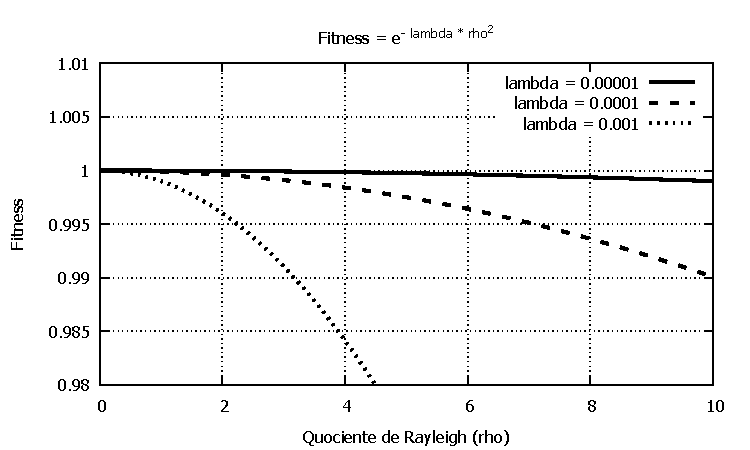
\includegraphics{figs/varios-fit-mono-zoom.pdf}
		\caption{Zoom próximo do pico}
		\label{fig:varios-fit-mono-zoom}
	\end{figure}
	
		
	$$
		\frac{df}{d\rho} = -2\lambda(\rho - \rho0)e^{-\lambda(\rho - \rho0)^2}
	$$
	
		
	\begin{figure}[htbp]
		\centering
			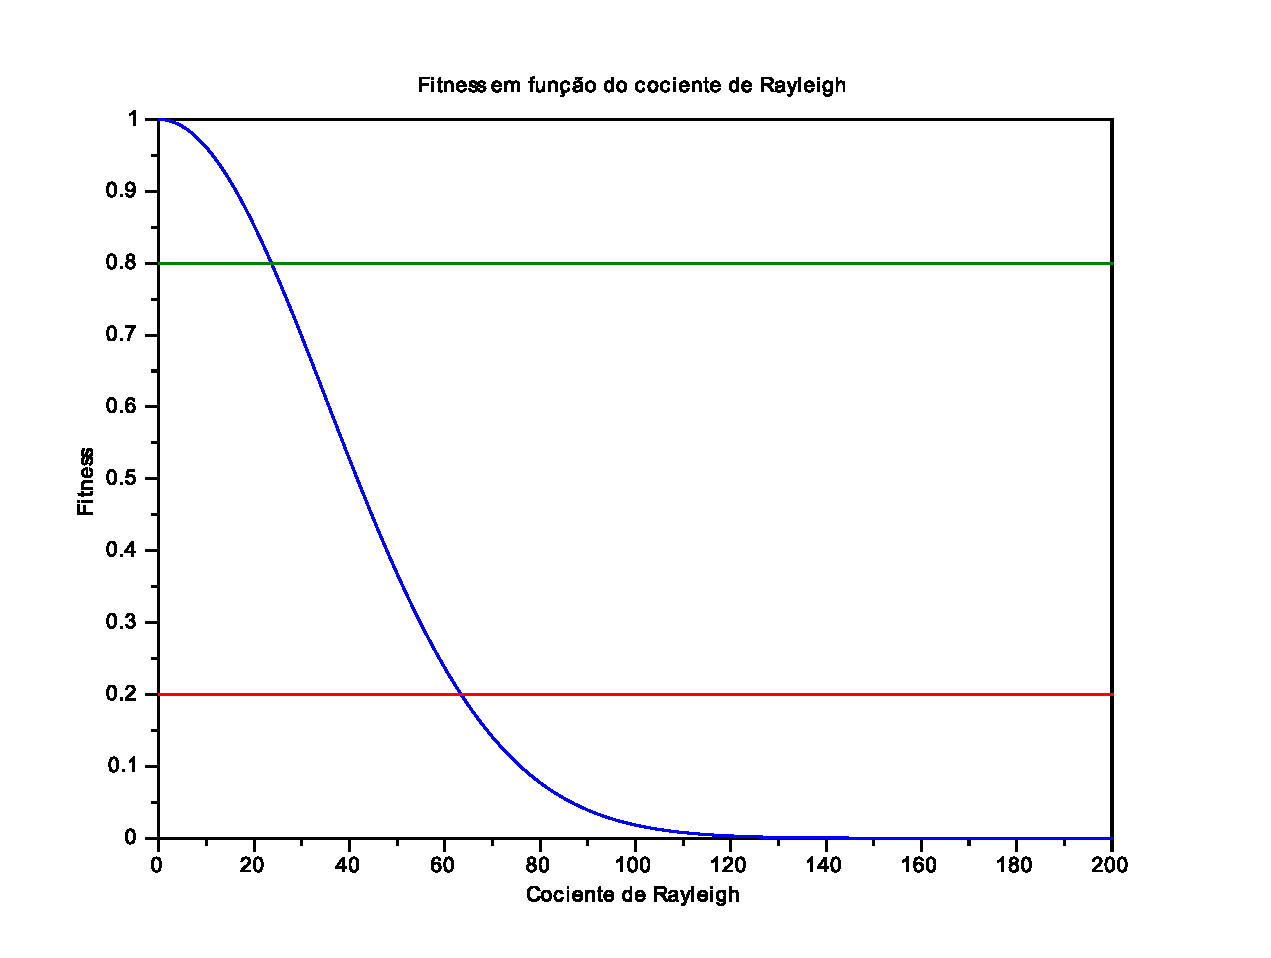
\includegraphics[width=0.90\textwidth]{figs/resultados/fitness_boaRegiao.pdf}
		\caption{Boa região para o fitness (entre as duas linhas)}
		\label{fig:fitness_boaRegiao}
	\end{figure}
	
	
	% Table generated by Excel2LaTeX from sheet 'Plan2'
\begin{tabular}{rr}

       \textit{rho} &          \textit{f} \\

      -0,1 &   0,999996 \\

     -0,09 &   0,999997 \\

     -0,08 &   0,999997 \\

     -0,07 &   0,999998 \\

     -0,06 &   0,999999 \\

     -0,05 &   0,999999 \\

     -0,04 &   0,999999 \\

     -0,03 &          1 \\

     -0,02 &          1 \\

     -0,01 &          1 \\

         0 &          1 \\

      0,01 &          1 \\

      0,02 &          1 \\

      0,03 &          1 \\

      0,04 &   0,999999 \\

      0,05 &   0,999999 \\

      0,06 &   0,999999 \\

      0,07 &   0,999998 \\

      0,08 &   0,999997 \\

      0,09 &   0,999997 \\

       0,1 &   0,999996 \\

\end{tabular}  
		
	
	\begin{figure}[pt]
	\centering
		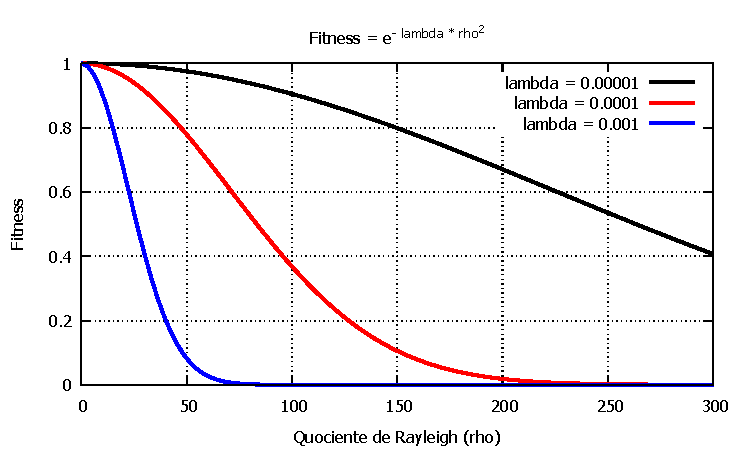
\includegraphics{figs/varios-fits-color.pdf}
	\caption{Fitness em função do lambda $-$ colorido}
	\label{fig:varios-fits-color}
\end{figure}

\begin{figure}[pb]
	\centering
		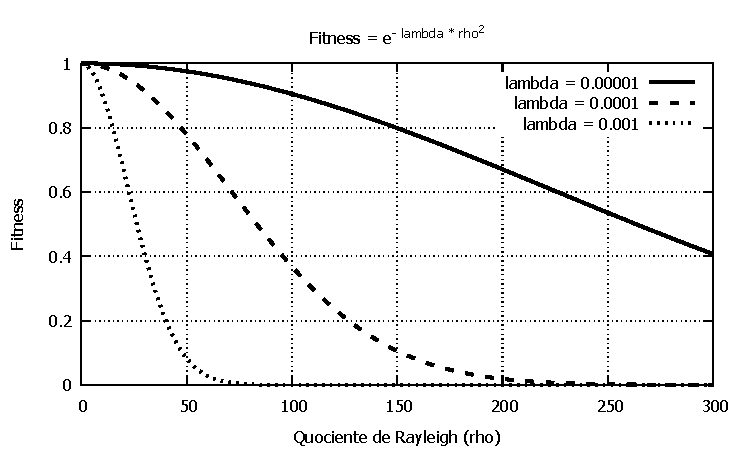
\includegraphics{figs/varios-fits-mono.pdf}
	\caption{Fitness em função do lambda}
	\label{fig:varios-fits-mono}
\end{figure}


% --- Finaliza a parte no bookmark do PDF, para que se inicie o bookmark na raiz ---
\bookmarksetup{startatroot}%

% ---- ELEMENTOS PóS-TEXTUAIS ----
\postextual

% ---- Referências bibliográficas ----
\bibliography{tese}

% ---- Apêndices ----
\begin{apendicesenv}
% Imprime uma página indicando o início dos apêndices
\partapendices

\chapter{Título do Apêndice A}

Texto aqui.
\chapter{Título do Apêndice B}

Texto aqui.

\end{apendicesenv}

% ---- Anexos ----
\begin{anexosenv}
% Imprime uma página indicando o início dos anexos
\partanexos

\chapter{Título do Anexo X}

Texto aqui.
\chapter{Título do Anexo Y}

Texto aqui.

\end{anexosenv}

% ---- INDICE REMISSIVO ----
\printindex

\end{document} 